\documentclass[10pt,twoside]{article}

\usepackage[T1]{fontenc}
\usepackage[utf8]{inputenc}
\usepackage{newtxtext,newtxmath}
\usepackage[margin=1in]{geometry}
\usepackage{microtype}
\usepackage{amsmath,mathtools}
\usepackage{graphicx}
\usepackage{booktabs}
\usepackage{tabularx}
\usepackage{array}
\usepackage{threeparttable}
\usepackage{caption}
\usepackage{enumitem}
\usepackage{xcolor}
\usepackage[authoryear,round]{natbib}
\usepackage{xurl}
\usepackage{hyperref}

\definecolor{paperblue}{HTML}{173A56}
\definecolor{linkblue}{HTML}{245E83}
\hypersetup{
  colorlinks=true,
  linkcolor=linkblue,
  citecolor=linkblue,
  urlcolor=linkblue,
  pdftitle={How Polymarket Probabilities Move},
  pdfauthor={Chronos Research Project},
  pdfsubject={Statistical analysis of recorded Polymarket probability histories},
  pdfkeywords={Polymarket, recorded probabilities, unchanged values, reversals, variance ratio}
}

\graphicspath{{figures/}}
\captionsetup{font=small,labelfont=bf,labelsep=period}
\setlength{\parindent}{1.2em}
\setlength{\parskip}{0pt}
\setlength{\emergencystretch}{2em}
\setcounter{secnumdepth}{3}
\setcounter{tocdepth}{2}
\newcolumntype{Y}{>{\raggedright\arraybackslash}X}
\newcolumntype{C}[1]{>{\centering\arraybackslash}p{#1}}

\title{\vspace{-1.5em}\textbf{How Polymarket Probabilities Move}\\[0.35em]
\large A Statistical Study of Unchanged Values, Sudden Moves, Reversals, and Variance over Time}
\author{Chronos Research Project}
\date{24 August 2026}

\begin{document}
\raggedbottom
\pagestyle{plain}
\maketitle
\thispagestyle{plain}

\begin{abstract}
We study sequences of probabilities saved by Polymarket. Each value is one recorded number at a known time. It need not be a transaction, an available quote, or the market's true probability. The main data contain 803,862 hourly observations from 562 contracts in 157 events. Tests on later events find four clear patterns. Many hourly changes are exactly zero. Long runs of unchanged values tend to continue. When two changes occur next to each other, their directions are more likely to be opposite than a simple independent model predicts. Finally, variation over 24 hours is much smaller than 24 times the variation over one hour. We model the next recorded change in three steps: whether the value moves, which direction it moves, and how far it moves. On 17,671 later observations from 27 events, a model using the current value and recent history had an average negative log likelihood of 2.870. The same model without recent history scored 3.116, and a smooth-change model scored 4.582; lower is better. These results describe the recorded sequence. They do not reveal exactly how beliefs or prices changed between two saved observations.
\end{abstract}

\noindent\textbf{Keywords:} prediction markets; stochastic processes; recorded probability changes; quiet periods; variance ratio; later-event testing.

\section{Introduction}

A saved probability can stay fixed for several reasons. The underlying probability may be stable. The displayed value may be rounded. The source may update only at certain times. These explanations are different, but they can produce the same recorded sequence. The data used here cannot separate them. We therefore begin with what was recorded and avoid assuming what happened between records.

The question is narrow: what probability model describes the next saved change in a Polymarket contract? Four facts matter. First, many hourly changes are exactly zero. Second, changes occur in groups. After a long unchanged run, another zero is much more likely than it is just after a change. Third, two consecutive nonzero changes point in opposite directions more often than an independent model with equally likely directions predicts. Fourth, the variance of a 24-hour change is much less than 24 times the variance of a one-hour change.

These facts suggest a three-part model. It first assigns a probability that the next saved value will move. If it moves, the model assigns probabilities to an increase and a decrease. It then describes the size of that change. The inputs are the current probability, time remaining, length of the current unchanged run, fraction of recent changes that were zero, and the direction and size of the previous nonzero change. We compare this model with simpler versions and with a model in which values change smoothly.

This is a description of the data, not an explanation of cause. The tests do not show why a contract moved, what information caused the move, or what happened inside an hour. The source also does not state whether each saved value is the last observed value, a midpoint, or another summary. Every conclusion in the paper is therefore about the saved sequence itself.

\section{What is being measured}

\subsection{Recorded values and the unobserved process}

Let $e$ identify an event, $i$ a contract within that event, and $t$ a regular observation time. The recorded YES probability is
\begin{equation}
  P_{e i t}\in[0,1].
  \label{eq:recorded-probability}
\end{equation}
There may be an unobserved probability $X_{e i}(s)$ that changes continuously between records. We do not know how it becomes the saved value $P_{e i t}$. We write that unknown relationship as
\begin{equation}
  P_{e i t}
  =\mathcal O_{e i t}\!\left(\{X_{e i}(s):s\le \tau_{e i t}\},R_{e i t}\right),
  \label{eq:observation-operator}
\end{equation}
Here $\tau_{e i t}$ is the time of the saved record, $R_{e i t}$ stands for any rounding or recording rules, and $\mathcal O_{e i t}$ stands for the unknown rule that turns the earlier path of $X$ into $P$. Equation~\eqref{eq:observation-operator} is bookkeeping, not a fitted model. We estimate neither $X$ nor $\mathcal O$. Everything below concerns $P$.

For two records exactly one hour apart, the change is
\begin{equation}
  Y_{e i,t+1}=\Delta P_{e i,t+1}=P_{e i,t+1}-P_{e i t}.
  \label{eq:increment}
\end{equation}
We do not call an irregular gap a one-hour change. We also restart all recent-history measurements after such a gap. Since a probability must remain between zero and one, a change cannot be smaller than $-P_{e i t}$ or larger than $1-P_{e i t}$.

We split each change into three parts:
\begin{equation}
  Y_{e i,t+1}=A_{e i,t+1}S_{e i,t+1}M_{e i,t+1},
  \label{eq:asm-decomposition}
\end{equation}
where
\begin{align}
  A_{e i,t+1}&=\mathbf 1\{Y_{e i,t+1}\ne0\}, \\
  S_{e i,t+1}&=\operatorname{sign}(Y_{e i,t+1})\in\{-1,+1\}\quad\text{when }A_{e i,t+1}=1, \\
  M_{e i,t+1}&=|Y_{e i,t+1}|\quad\text{when }A_{e i,t+1}=1.
\end{align}
$A$ says whether the value changed, $S$ gives its direction, and $M$ gives its absolute size. Their product reconstructs the recorded change. This separation matters because a model can be right about long unchanged runs while being wrong about the direction or size of the changes that do occur.

\subsection{Four quantities that describe movement}

Let $\mathcal T_e$ be the set of valid regular changes in event $e$. The fraction that are exactly zero is
\begin{equation}
  \widehat Z_e
  =\frac{1}{|\mathcal T_e|}\sum_{(i,t)\in\mathcal T_e}\mathbf 1\{Y_{e i,t+1}=0\}.
  \label{eq:zero-share}
\end{equation}
A continuous distribution assigns probability zero to any one exact number. A large observed fraction at exactly zero therefore requires the model to give ``no recorded change'' its own probability, or to model a recording rule such as rounding.

Let the quiet duration $Q_{e i t}$ be the number of consecutive regular changes equal to zero up to time $t$. We compare the chance of a move after at least 24 unchanged hours with the chance of a move immediately after another move:
\begin{equation}
  \widehat R^{\mathrm{quiet}}_e
  =\frac{
    \widehat{\Pr}_e(A_{t+1}=1\mid Q_t\ge24)
  }{
    \widehat{\Pr}_e(A_{t+1}=1\mid A_t=1)
  }.
  \label{eq:quiet-ratio}
\end{equation}
A ratio below one means that long unchanged runs tend to continue. The test was fixed in advance and asked whether the ratio was below $0.50$.

When two neighboring changes are both nonzero, their reversal fraction is
\begin{equation}
  \widehat R^{\mathrm{sign}}_e
  =\frac{
  \sum_{(i,t)\in\mathcal T_e}
  A_{e i t}A_{e i,t+1}\mathbf 1\{S_{e i,t+1}\ne S_{e i t}\}
  }{
  \sum_{(i,t)\in\mathcal T_e}A_{e i t}A_{e i,t+1}
  }.
  \label{eq:reversal-share}
\end{equation}
If increases and decreases were equally likely and independent from one hour to the next, this fraction would be $0.50$.

For a period of $h$ hours, the variance ratio is
\begin{equation}
  \widehat{\mathrm{VR}}_e(h)
  =\frac{\widehat{\operatorname{Var}}_e(P_{t+h}-P_t)}
  {h\,\widehat{\operatorname{Var}}_e(P_{t+1}-P_t)}.
  \label{eq:variance-ratio}
\end{equation}
The numerator is the observed variance of an $h$-hour change. The denominator is what that variance would be if one-hour changes were independent and had a constant variance. Under that simple model, $\mathrm{VR}(h)=1$.

If the variance and covariance of one-hour changes are approximately stable over the period being examined, the same ratio can be written as
\begin{equation}
  \mathrm{VR}(h)
  =1+2\sum_{k=1}^{h-1}\left(1-\frac{k}{h}\right)\frac{\gamma(k)}{\gamma(0)}.
  \label{eq:vr-covariance}
\end{equation}
Here $\gamma(k)$ is the covariance between changes $k$ hours apart. Negative covariance at short lags pulls the ratio below one. We use this equation to explain the measurement; we do not assume that every contract has constant behavior over its full life.

\section{Data and testing order}

\subsection{Evidence sets}

The main data contain 803,862 hourly records from 562 contracts in 157 events. We keep related contracts in the same event because they may react to the same information. Table~\ref{tab:evidence} shows exactly which data are used for each part of the paper.

\begin{table}[htbp]
\centering
\caption{Evidence sets used in the analysis.}
\label{tab:evidence}
\small
\begin{tabularx}{\textwidth}{@{}p{0.19\textwidth}Y Y@{}}
\toprule
Evidence set & Contents & Role \\
\midrule
Main group & 803,862 hourly records; 562 contracts; 157 events & Measure the process, fit models, and test them in time order \\
Later group & 29 later events; 27 eligible for the fixed one-hour models & Compare selected models without fitting them again \\
Five-minute group & 19,258 official history records from 10 contracts selected before their values were inspected & Check whether the patterns are caused only by hourly sampling \\
Separate reversal group & 6,174 non-overlapping large-change cases; 410 contracts; 128 test events & Check the direction-reversal result on different events \\
Fixed move/no-move run & 100 declared cases; 65 could be scored under the fixed rules & Check both accuracy and the fraction of cases the implementation can handle \\
\bottomrule
\end{tabularx}
\end{table}

One observation is one saved probability for one contract at one time. It is not necessarily a transaction. In this paper, \emph{zero} means no difference between two neighboring saved values, \emph{move} means any nonzero difference, and \emph{reversal} means that two neighboring nonzero differences have opposite directions. A recorded move does not prove that the unobserved process $X$ jumped suddenly.

\subsection{Training on earlier events and testing on later ones}

Every model input is calculated from records that exist before the value being predicted. Models are fitted on earlier complete events and tested on later complete events. Numerical transformations are also fitted using only the earlier events. No input uses the contract's final outcome. This time ordering prevents the answer from leaking into the model.

We use two scores. The first checks predictions of a yes-or-no outcome, such as whether the next value moves. If the observed answer is $y_{e j}\in\{0,1\}$ and the predicted probability is $q_{e j}$, the Brier score is the mean squared error \citep{brier1950}:
\begin{equation}
  \mathrm{BS}_e
  =\frac{1}{n_e}\sum_{j=1}^{n_e}(q_{e j}-y_{e j})^2,
  \qquad
  \overline{\mathrm{BS}}
  =\frac{1}{|\mathcal E|}\sum_{e\in\mathcal E}\mathrm{BS}_e.
  \label{eq:brier}
\end{equation}
The second score checks the complete predicted distribution of the next change. Let $Q_{e j}$ be that distribution, and let $B(Y_{e j})$ be the recorded interval that contains the change that actually occurred. Negative log likelihood (NLL) penalizes a model when it assigns little probability to what happened:
\begin{equation}
  \mathrm{NLL}_e
  =-\frac{1}{n_e}\sum_{j=1}^{n_e}\log Q_{e j}\!\left(B(Y_{e j})\right),
  \qquad
  \overline{\mathrm{NLL}}
  =\frac{1}{|\mathcal E|}\sum_{e\in\mathcal E}\mathrm{NLL}_e.
  \label{eq:nll}
\end{equation}
Lower values are better for both scores. We first calculate a score inside each event and then average the event scores. This gives a small event and a large event equal weight instead of allowing the event with the most records to dominate the result.

Uncertainty is also calculated with whole events. A bootstrap sample draws events, not individual rows, so related contracts stay together. Because testing many claims makes a chance result more likely, the four main process tests use the Holm correction. The two retained model comparisons use the stricter Bonferroni correction across all 37 recorded statistical analyses. The audit lists 90 executions for 48 distinct analyses, including failed runs and reruns \citep{chronos2026audit}.

\section{What the recorded contracts do}

\subsection{Four tests on later events}

Table~\ref{tab:process-results} reports the four tests. Each comparison value was chosen before the later data were examined. The $0.50$ direction comparison follows from independent, equally likely increases and decreases. The other comparison values are deliberately cautious cutoffs, not laws of probability.

\begin{table}[htbp]
\centering
\caption{Four measurements averaged across later events.}
\label{tab:process-results}
\small
\setlength{\tabcolsep}{4pt}
\begin{tabular}{@{}lccccc@{}}
\toprule
Measure & Mean & 95\% interval & Fixed comparison & Events & Holm $p$ \\
\midrule
Exact-zero share & 43.81\% & 38.71\% to 49.52\% & above 20\% & 25/26 & 0.00000161 \\
Sign-reversal share & 58.45\% & 55.53\% to 61.41\% & above 50\% & 21/26 & 0.00249 \\
Long-quiet/active ratio & 7.36\% & 5.23\% to 9.65\% & below 50\% & 7/7 & 0.00781 \\
$\mathrm{VR}(24)$ & 32.40\% & 24.97\% to 40.43\% & below 75\% & 24/26 & 0.0000157 \\
\bottomrule
\end{tabular}
\end{table}

Across events, 43.81\% of hourly changes were exactly zero on average. A Gaussian model assigns no probability to one exact value, including zero. A useful model for these data must therefore assign a separate probability to no recorded change, although that probability can differ across contracts and groups of events.

The long-quiet ratio was 7.36\%. After at least 24 unchanged hourly records, the chance of a change in the next hour was about 7\% of the chance observed immediately after a change. Knowing only the current probability is therefore not enough. The length of the unchanged run also tells us something about whether the next value will move.

The average reversal fraction was 58.45\%. Under the independent equal-direction comparison, it would be 50\%. A separate test found the same tendency. After a change of at least two probability points and a one-record delay, a model using six facts about the current value and the earlier change reduced the event-average Brier score from 0.2522 to 0.2390. This test covered 6,174 cases in 128 later events. The 95\% whole-event interval for the score reduction was 0.0051 to 0.0214. The richer model had the lower score in 87 of 128 events, with an adjusted $p$-value of 0.00109.

Finally, $\mathrm{VR}(24)$ was 0.3240. The variance of a 24-hour change was only about 32\% of the value obtained by multiplying the one-hour variance by 24. Frequent reversals help cancel earlier changes, and long unchanged runs mean that 24 clock hours do not contain 24 independent chances to move. We use the variance ratio only as this comparison. We do not assume that the distribution stays constant over the full life of every contract; for the classical formula, see \citet{lo1988}.

\begin{figure}[htbp]
\centering
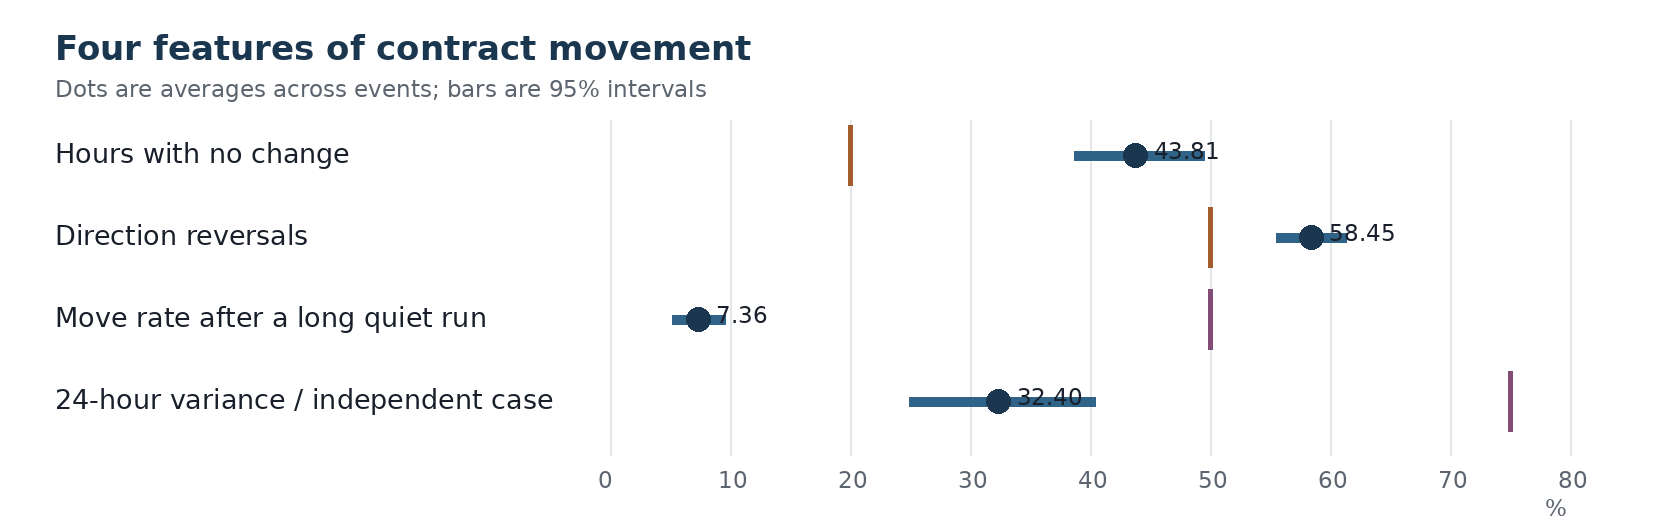
\includegraphics[width=0.94\textwidth]{process_signatures.png}
\caption{Average results across later events. Horizontal bars show 95\% intervals obtained by resampling whole events. Vertical markers show the comparison value fixed in advance for each test.}
\label{fig:process-signatures}
\end{figure}

\subsection{Checking the same patterns every five minutes}

Hourly records might create false patterns by hiding several changes inside each hour. We therefore repeated the measurements on ten contracts recorded every five minutes. These contracts were selected before their values were examined. The data contain 19,258 official history records and 19,012 regular five-minute changes. Of these changes, 78.00\% were zero, 67.87\% of neighboring nonzero changes reversed direction, and the 24-hour variance ratio was 0.067.

Ten contracts are too few to estimate the behavior of all Polymarket contracts. This check answers a smaller question: the exact zeros, reversals, and low variance ratio do not disappear when the interval falls from one hour to five minutes. Hourly sampling cannot be the whole explanation. The test still cannot tell whether rounding, irregular source updates, or the unobserved process produced the patterns.

\section{A model for the next saved change}

\subsection{No change, direction, and size in one formula}

Let $\mathcal F_{e i t}$ contain everything recorded up to time $t$. The distribution of the next change is
\begin{equation}
\begin{split}
  Q_{e i t}(dy)
  ={}&(1-\pi_{e i t})\,\delta_0(dy) \\
  &+\pi_{e i t}\left[
  \rho_{e i t} f_{+,e i t}(y)\mathbf 1_{(0,\,1-P_{e i t}]}(y)
  +(1-\rho_{e i t}) f_{-,e i t}(-y)\mathbf 1_{[-P_{e i t},\,0)}(y)
  \right]dy,
  \label{eq:mixture-law}
\end{split}
\end{equation}
where
\begin{align}
  \pi_{e i t}&=\Pr(A_{e i,t+1}=1\mid\mathcal F_{e i t}), \\
  \rho_{e i t}&=\Pr(S_{e i,t+1}=+1\mid A_{e i,t+1}=1,\mathcal F_{e i t}),
\end{align}
$\pi_{e i t}$ is the probability that the next saved value changes. If it changes, $\rho_{e i t}$ is the probability that it increases. The symbol $\delta_0$ assigns a separate probability to exactly zero. The functions $f_+$ and $f_-$ describe the sizes of increases and decreases. Their allowed ranges stop at zero and one, so the predicted probability cannot leave $[0,1]$. In plain terms, Equation~\eqref{eq:mixture-law} asks three questions in order: does the value move, in which direction, and by how much? Similar factorizations are used for the timing and size of events \citep{hawkes1971,bacry2013}. This discrete-time formula does not reconstruct what happens between saved observations.

We fit those three parts as follows:
\begin{align}
  \operatorname{logit}(\pi_{e i t})
  &=\alpha_A+x^{(A)\top}_{e i t}\beta_A, \\
  \operatorname{logit}(\rho_{e i t})
  &=\alpha_S+x^{(S)\top}_{e i t}\beta_S, \\
  \log M_{e i,t+1}\mid A_{e i,t+1}=1,S_{e i,t+1}
  &\sim\mathcal N\!\left(\alpha_M+x^{(M)\top}_{e i t}\beta_M,\sigma_M^2\right),
  \label{eq:component-models}
\end{align}
The first logistic equation predicts whether a change occurs. The second predicts an increase, given that a change occurs. The third models the logarithm of the change size with a normal distribution. Scoring uses probability intervals that match the precision of the saved values. The normal assumption applies only to the logarithm of size after a nonzero change. It does not make the full distribution Gaussian: the full distribution still contains many exact zeros and combines observations from contracts with different levels of activity.

\subsection{What the model knows at each observation}

The available inputs are collected in the vector
\begin{equation}
  x_{e i t}=\left(
  P_{e i t},\ d_{e i t},\ \ell_{e i t},\ T_{e i t},\
  \log(1+Q_{e i t}),\ Z^{(24)}_{e i t},\ S^{-}_{e i t},\ \log M^{-}_{e i t}
  \right),
  \label{eq:state-vector}
\end{equation}
where
\begin{align}
  d_{e i t}&=\min(P_{e i t},1-P_{e i t}), \\
  \ell_{e i t}&=\log\!\left(\frac{\widetilde P_{e i t}}{1-\widetilde P_{e i t}}\right),
  \qquad \widetilde P_{e i t}=\min(0.995,\max(0.005,P_{e i t})), \\
  Z^{(24)}_{e i t}&=\frac{1}{24}\sum_{k=0}^{23}\mathbf 1\{Y_{e i,t-k}=0\}.
\end{align}
The first three entries describe the current probability in different ways. $P$ is the probability itself, $d$ is its distance from the nearest boundary, and $\ell$ is its log odds after clipping values very close to zero or one. $T$ is time until the recorded close. $Q$ is the length of the current unchanged run. $Z^{(24)}$ is the fraction of the previous 24 changes that were zero. $S^{-}$ and $M^{-}$ are the direction and size of the last nonzero change.

The move/no-move equation uses the current probability and the unchanged-run measurements. The direction equation also uses the direction of the previous nonzero change. The size equation also uses the previous nonzero size. Each input therefore has a stated purpose, and every input is known before the change being modeled.

\subsection{The four models being compared}

We compare four models, adding one source of information at a time:
\begin{enumerate}[leftmargin=2em,itemsep=0.25em]
  \item \textbf{Smooth-change model.} The next change follows a Gaussian distribution centered at zero. Its scale depends on the current probability and time remaining, and it shrinks near zero and one. Because the distribution is continuous, it assigns no separate probability to an exact zero.
  \item \textbf{Move/no-move model without context.} The model has a separate probability for no change, followed by distributions for direction and size. These probabilities are estimated from earlier events but do not use the current probability or recent history.
  \item \textbf{Current-value model.} The three parts also use the current probability and time remaining.
  \item \textbf{Current-value-and-history model.} The model also uses the length of the unchanged run, the direction of the previous nonzero change, and its size.
\end{enumerate}
The last comparison tells us whether recent history adds information after the current value and time remaining are already known.

\section{Which model matched later events}

\subsection{The full distribution of the next change}

During model development, we made 566,501 predictions in time order across 113 events. After choosing the four models, we fixed them and made 17,671 further predictions on 27 eligible later events. Table~\ref{tab:model-scores} reports NLL after giving every event equal weight. NLL measures how much probability a model assigned to the change that occurred; lower values are better.

\begin{table}[htbp]
\centering
\caption{Negative log likelihood for four process descriptions. Lower values are better.}
\label{tab:model-scores}
\small
\begin{tabularx}{\textwidth}{@{}Y C{0.9in} C{0.9in} Y@{}}
\toprule
Model & Development NLL & Later NLL & Statistical content \\
\midrule
Smooth change & 3.578 & 4.582 & Continuous changes; no separate probability for exact zero \\
Move/no-move without context & 2.214 & 3.240 & Separate zero, direction, and size; no current information \\
Current value & 2.104 & 3.116 & Adds current probability and time remaining \\
Current value and history & 1.941 & 2.870 & Adds quiet duration, previous direction, and previous size \\
\bottomrule
\end{tabularx}
\end{table}

Compared with the current-value model, adding recent history lowered NLL on later events by
\begin{equation}
  \frac{3.116-2.870}{3.116}=0.0788,
  \label{eq:nll-reduction}
\end{equation}
or 7.88\%. It had the lower score in every one of the 27 events. All four models scored worse on the later events than during development. The later data were therefore harder to describe, but the order of the four models did not change.

\begin{figure}[htbp]
\centering
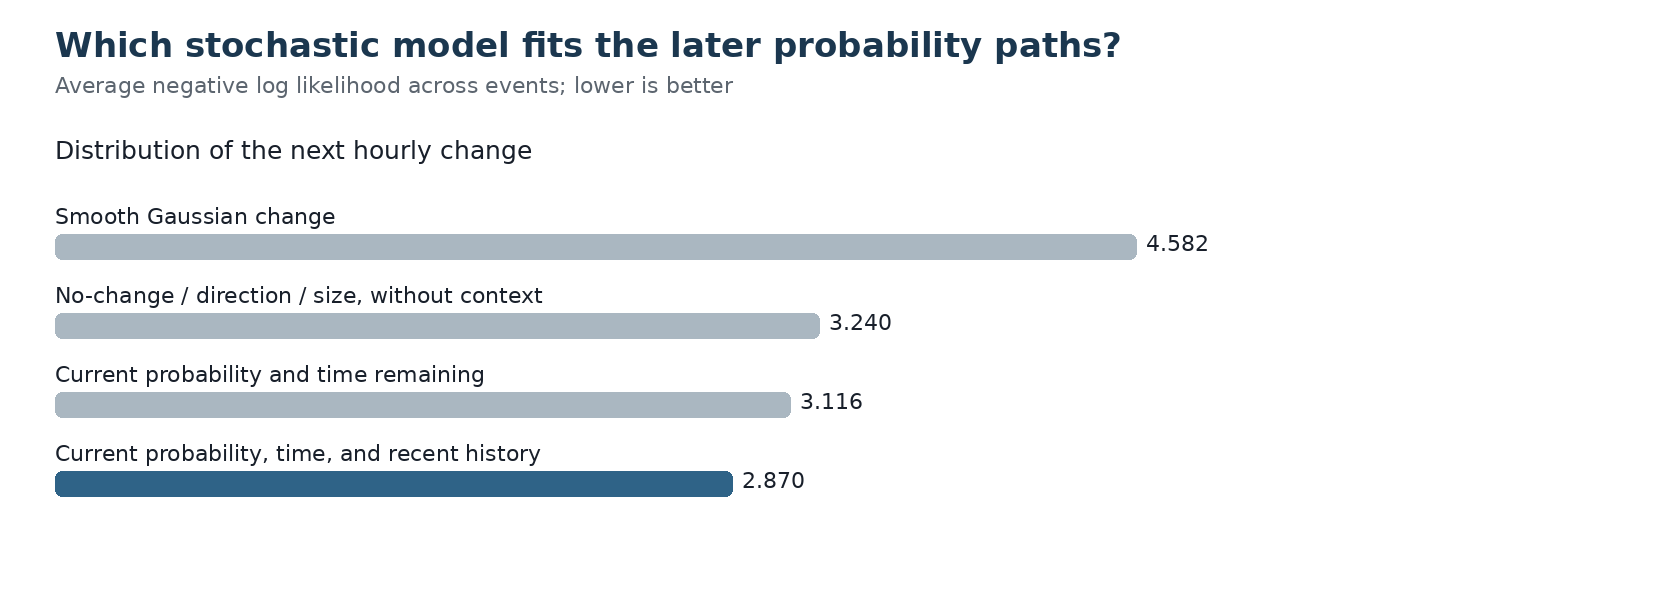
\includegraphics[width=0.92\textwidth]{model_scores.png}
\caption{Scores on later events. The left panel checks the full distribution of the next change using event-average NLL. The right panel checks only whether the next saved value changed, using event-average Brier score. Lower values are better.}
\label{fig:model-scores}
\end{figure}

\subsection{Whether the next value changes}

We next examine only $A_{e i,t+1}$, the yes-or-no question of whether the next value changes. The simpler logistic model uses the current probability, its distance from zero or one, and its clipped log odds. The history model adds the length of the unchanged run and the fraction of the previous 24 changes that were zero. On the later events, the event-average Brier score fell from 0.2611 to 0.1739:
\begin{equation}
  \frac{0.2611-0.1739}{0.2611}=0.3338.
  \label{eq:brier-reduction}
\end{equation}
This is a 33.38\% reduction in mean squared probability error. The history model had the lower score in all 27 events. Resampling whole events gave a 95\% interval of 0.0716 to 0.1035 for the absolute score reduction. After correcting for all 37 recorded statistical analyses, the $p$-value from the event wins was 0.000000276. Among the recent-history inputs, the length of the unchanged run produced the largest and most consistent improvement.

One separate implementation was fixed in advance and declared for 100 cases, but its required data were available for only 65. Its Brier score on those 65 cases was 0.189, better than the fixed maximum of 0.200. Its coverage was only 65\%, far below the required 95\%. We cannot simply ignore the missing 35 cases because missing data may be related to a contract's history. This result says that the implementation failed to cover its declared cases. It does not undo the result on the 27 complete later events, but it prevents us from claiming that this implementation works wherever it was intended to run.

\section{What the results say about the process}

The recorded probability is bounded between zero and one. Its next value often stays exactly fixed, so zero needs its own probability in the model. The chance of a change depends on the current probability, time remaining, and how long the value has already been unchanged. When changes do occur, their directions tend to reverse over short periods. Their sizes also depend on the current probability and on the size of the previous nonzero change.

The current probability $P_t$ alone does not contain all useful information about the next recorded value. In the language of stochastic processes, $P_t$ by itself is not an adequate first-order Markov state: recent history still improves the next-step distribution. A more useful summary is
\begin{equation}
  \Xi_t=(P_t,T_t,Q_t,Z_t^{(24)},S_t^{-},M_t^{-})
  \label{eq:augmented-state}
\end{equation}
This vector contains the current probability, time remaining, length and frequency of recent unchanged observations, and the direction and size of the last nonzero change. It is a useful finite summary of the recorded past. The tests do not prove that it is the smallest possible summary or that it captures every relevant part of history.

Three simple descriptions fit the data poorly: independent Gaussian changes, a model with a constant chance of changing, and a model that knows the current probability but forgets recent changes. The results do not tell us which unseen mechanism produced the records. Long unchanged runs and groups of moves could arise because one move makes another more likely, because the chance of a move depends on the time since the last one, because the source updates irregularly, or because values are rounded. The saved histories alone cannot distinguish these explanations.

Different events also behave differently. Every model scored worse on the later events, the fraction of exact zeros changed between groups, and only seven later events had enough observations to estimate the long-quiet ratio. The same model structure works across groups more reliably than one fixed set of numerical coefficients does.

\section{Limitations and next measurements}

The main data contain one record per hour, so they show nothing inside an hour. The source does not define the saved field precisely enough to tell whether it is the last observation or another summary. The five-minute check shortens the hidden interval but contains only ten contracts. It shows that hourly sampling is not the whole explanation; it does not tell us which other explanation is correct.

The later group was not used to fit the earlier model. It was then used for several reported analyses, so it should now be treated as used data, not as an untouched test set for future work. Grouping related contracts inside events handles the clearest relationships, but two events with different names may still respond to some of the same information.

The smooth-change model is deliberately simple. Its poor score does not rule out every continuously changing process, especially if we observe that process only after rounding or irregular updates. The low variance ratio also does not mean that behavior is constant over time. The direct claims are narrower: exact zeros are common; long unchanged runs tend to continue; short-run changes often reverse; variance grows slowly with the observation period; the current value matters; recent history matters; and the strength of these patterns differs across events.

Three further measurements would help separate the remaining explanations. First, a longer data set recorded at several fixed intervals $\Delta$ would show how the zero fraction $Z(\Delta)$, reversal fraction $R^{\mathrm{sign}}(\Delta)$, and variance ratio $\mathrm{VR}(h;\Delta)$ change as observations become more frequent. Second, fixed contract categories would let a multilevel model measure how much behavior differs between events and categories. Third, matching public announcements to the probability histories would separate changes near scheduled information from changes at ordinary times. These extensions can keep the same rule used here: fit on earlier whole events and test on later whole events.

\section{Conclusion}

Recorded Polymarket probabilities often remain exactly unchanged for long periods and then move several times close together. Neighboring nonzero changes reverse direction more often than an independent equal-direction model predicts. Over 24 hours, variance is much smaller than 24 times the one-hour variance. The current probability matters, and so does its recent history.

The best tested model is Equation~\eqref{eq:mixture-law}. It first assigns a separate probability to no change. If a change occurs, it describes the direction and size. The length of the current unchanged run gives the largest improvement. The previous direction and size add smaller but repeated improvements. This model also performs best on later events, although every model finds those events harder.

The paper does not attach one continuous-time explanation to these findings. What can be said directly is simple: the recorded value stays between zero and one, is often exactly unchanged, depends on how long it has been unchanged, retains information from earlier changes, and behaves differently across events. Finding the mechanism underneath the saved observations requires better information about how and when those observations were produced.

\begin{thebibliography}{9}

\bibitem[Bacry et al.(2013)Bacry, Delattre, Hoffmann, and Muzy]{bacry2013}
Bacry, E., Delattre, S., Hoffmann, M., and Muzy, J. F. (2013).
Modelling microstructure noise with mutually exciting point processes.
\emph{Quantitative Finance}, 13(1), 65-77.

\bibitem[Brier(1950)]{brier1950}
Brier, G. W. (1950).
Verification of forecasts expressed in terms of probability.
\emph{Monthly Weather Review}, 78(1), 1-3.

\bibitem[Chronos Research Project(2026)]{chronos2026audit}
Chronos Research Project (2026).
\emph{Polymarket Paper Acceptance Audit}.
Audit identity: \nolinkurl{paper-audit-report:e8ed21a7f08e0e35c8277138515f0cad1cf0d84f0fe6fca438aa380f0fa2d910}.

\bibitem[Hawkes(1971)]{hawkes1971}
Hawkes, A. G. (1971).
Spectra of some self-exciting and mutually exciting point processes.
\emph{Biometrika}, 58(1), 83-90.

\bibitem[Lo and MacKinlay(1988)]{lo1988}
Lo, A. W., and MacKinlay, A. C. (1988).
Stock market prices do not follow random walks: Evidence from a simple specification test.
\emph{Review of Financial Studies}, 1(1), 41-66.

\end{thebibliography}

\end{document}
